\documentclass[
    12pt,
    openright,
    twoside,
    a4paper,
    english,
    spanish,
    brazil,
    ]{abntex2}

% ---
% PACOTES
% ---

\usepackage{cmap}
\usepackage{lmodern}
\usepackage[T1]{fontenc}
\usepackage[utf8]{inputenc}
\usepackage{lastpage}
\usepackage{indentfirst}
\usepackage{color}
\usepackage{graphicx}
\usepackage{lipsum}
\usepackage[brazilian,hyperpageref]{backref}
\usepackage[alf]{abntex2cite}

\renewcommand{\backrefpagesname}{Citado na(s) página(s):~}
\renewcommand{\backref}{}
\renewcommand*{\backrefalt}[4]{
    \ifcase #1 %
        Nenhuma citação no texto.%
    \or
        Citado na página #2.%
    \else
        Citado #1 vezes nas páginas #2.%
    \fi}%
% ---


% ---
% Informações de dados para CAPA e FOLHA DE ROSTO
% ---
\titulo{Protótipo de baixo custo para integração do AVS em sistemas embarcados}
\autor{Guilherme Vinícius Barbosa Pereira Amorim}
\local{Belo Horizonte}
\data{2022}
\orientador{Prof. Ricardo de Oliveira Duarte}
%\coorientador{Prof. }
\instituicao{%
  Universidade Federal de Minas Gerais -- UFMG
  \par
  Escola de Engenharia
  \par
  Curso de Graduação em Engenharia Elétrica}
\tipotrabalho{Trabalho de Conclusão de Curso}

% O preambulo deve conter o tipo do trabalho, o objetivo, o nome da instituição e a área de concentração 
\preambulo{Monografia apresentada durante o Seminário dos Trabalhos de Conclusão do Curso de Graduação em Engenharia Elétrica da UFMG, como parte dos requisitos necessários à obtenção do título de Engenheiro Eletricista.}
% ---

% ---
% Configurações de aparência do PDF final

% alterando o aspecto da cor azul
\definecolor{blue}{RGB}{41,5,195}

% informações do PDF
\makeatletter
\hypersetup{
         %pagebackref=true,
        pdftitle={\@title},
        pdfauthor={\@author},
        pdfsubject={\imprimirpreambulo},
        pdfcreator={LaTeX with abnTeX2},
        pdfkeywords={abnt}{latex}{abntex}{abntex2}{trabalho acadêmico},
        colorlinks=true,
        linkcolor=blue,
        citecolor=blue,
        filecolor=magenta,
        urlcolor=blue,
        bookmarksdepth=4
}
\makeatother
% ---

% ---
% Espaçamentos entre linhas e parágrafos
% ---

% O tamanho do parágrafo é dado por:
\setlength{\parindent}{1.3cm}

% Controle do espaçamento entre um parágrafo e outro:
\setlength{\parskip}{0.2cm}

% ---
% compila o índice
% ---
\makeindex
% ---

% ----
% Início do documento
% ----
\begin{document}

% Retira espaço extra obsoleto entre as frases.
\frenchspacing

% ----------------------------------------------------------
% ELEMENTOS PRÉ-TEXTUAIS
% ----------------------------------------------------------
% \pretextual

% ---
% Capa
% ---
\imprimircapa
% ---

% ---
% Folha de rosto
% ---
\imprimirfolhaderosto
% ---

% ---
% Dedicatória
% ---
\begin{dedicatoria}
\end{dedicatoria}
% ---

% ---
% Agradecimentos
% ---
\begin{agradecimentos}
\end{agradecimentos}
% ---

% ---
% inserir o sumario
% ---
\pdfbookmark[0]{\contentsname}{toc}
\tableofcontents*
\cleardoublepage
% ---

% ----------------------------------------------------------
% ELEMENTOS TEXTUAIS
% ----------------------------------------------------------
\textual

% ----------------------------------------------------------
% Capítulo 1 - Introdução
% ----------------------------------------------------------
\chapter{Introdução}
Atualmente o termo ‘sistemas embarcados’ não está muito presente no cotidiano brasileiro, mas essa tecnologia é responsável por fornecer equipamentos inteligentes como semáforos de trânsito, relógios, respiradores mecânicos, roteadores e aparelhos de ar-condicionado, por exemplo. Em termos simples, pode-se definir um sistema embarcado como um dispositivo controlado por um computador encapsulado. Ou seja, um sistema embarcado é na verdade um sistema microprocessado. Dentre as principais vantagens de sistemas embarcados, destaca-se o baixo custo, a eficiência e a facilidade de programação (NORLETO, 2020).

O primeiro sistema embarcado é o AGC (Apollo Guidance Computer). Ele foi desenvolvido nos EUA por Charles Stark Draper do MIT em 1966 (EMBARCADOS, 2014). Desde então, os sistemas embarcados ficaram mais acessíveis, mais velozes e mais compactos.

Com o passar dos anos, novas tecnologias foram adicionadas à sistemas embarcados, como por exemplo o Wifi, o bluetooth etc. Na última década foi observado a acensão de assistentes virtuais como a Alexa e o Google Assistent. A Alexa foi criada em 2014 e apareceu pela primeira vez como parte das caixas de som. Hoje a Alexa, a partir de comandos de voz, pode realizar pesquisas, mandar executar uma lista de músicas, disparar um alarme etc (VIGLIAROLO, 2017). Segundo o site oficial da Amazon Alexa (2022), o serviço permite a conexão com dispositivos, efetuar comandos por voz, interpretá-los e tomar uma ação correspondente. Isso tudo acontece por meio do Web Service da Amazon (AWS).

Visto que a tecnologia AWS e AVS (Alexa Voice Service) é recente, ainda não se observa a fácil e barata integração das assistentes de voz à sistemas embarcados. Existem hoje no mercado grandes empresas, como a STMicroeletronics, que produzem documentação e kits com o fim padronizar e facilitar o desenvolvimento de sistemas embutidos. Contudo, poucos exemplos são encontrados de como integrar assistentes pessoais a esses sistemas.

Diante do que foi dito, este trabalho se propõe permitir a fácil integração de sistemas embarcados à tecnologia AVS.
\section{Objetivos}
Este trabalho tem o objetivo de criar um protótipo de baixo custo que permite a fácil integração da assistente de voz Alexa (AVS) em sistemas embarcados.

Os seus objetivos específicos são:
\begin{alineas}
	\item suporte à rede Wifi IEEE 802.11 (2,4 GHz);
	\item detecção de palavra de ativação ("Alexa");
	\item responder o usuário por voz;
	\item ser configurado pelo aplicativo Amazon Alexa;
	\item criação de um Application Note.
\end{alineas}
\section{Estrutura}
O trabalho será apresentado em cinco capítulos. O capítulo 1 apresenta a introdução e os objetivos. O capítulo 2 apresenta o referencial teórico, contextualizando o projeto e citando trabalhos correlatos. O capítulo 3 contém o desenvolvimento do trabalho, apresentando requisitos funcionais e não-funcionais, ferramentas utilizadas e a implementação. O capítulo 4 expõe e faz a análise dos resultados. O capítulo 5, por fim, conclui o trabalho listando vantagens e desvantagens do protótipo, e as sugestões para trabalhos futuros.

% ----------------------------------------------------------
% Capítulo 2 - Referencial teórico
% ----------------------------------------------------------
\chapter{Referencial teórico}
\section{Computação em nuvem com a AWS}
A Amazon Web Services, Inc. (AWS) é uma empresa subsidiária da Amazon responsável por fornecer a seus clientes plataformas para a computação em nuvem sob demanda via Internet. Empresas fazem uso desse serviço para a criação e execução de aplicações virtuais sem um custo inicial, uma vez que a AWS tem o  \textit{pay-as-you-go} como modelo de precificação. Ou seja, o cliente faz o pagamento conforme o uso (AWS, 2019). Em 2022, a AWS é capaz de oferecer a seus clientes mais de duzentos serviços em nuvem nas áreas de tecnologias de computação, banco de dados, \textit{machine learning}, inteligência artificial etc.

Ademais, a AWS conta com 84 zonas de disponibilidade em 26 regiões geográficas. Esse modelo de região e zona de disponibilidade da AWS foi reconhecido pelo Gartner, empresa de pesquisa e consultoria em tecnologia da informação (TI), como o método recomendado para executar aplicativos corporativos que exigem alta disponibilidade (AWS, 2022).

Dentre os diversos serviços fornecidos pela AWS, o projeto fará uso do \textit{AWS Lambda} e do \textit{AWS IoT} para a integração da AVS em sistemas embutidos. A \autoref{fig_logo_aws} mostra os logos da AWS e da amazon alexa, e dos serviços AWS lambda e AWS Iot. A \autoref{fig_project_diagram} mostra o diagrama de integração dos serviços AWS e da amazon alexa no projeto.

\begin{figure}[htb]
	\caption{\label{fig_project_diagram}Diagrama de uso dos serviços AWS e AVS no projeto.}
	\begin{center}
		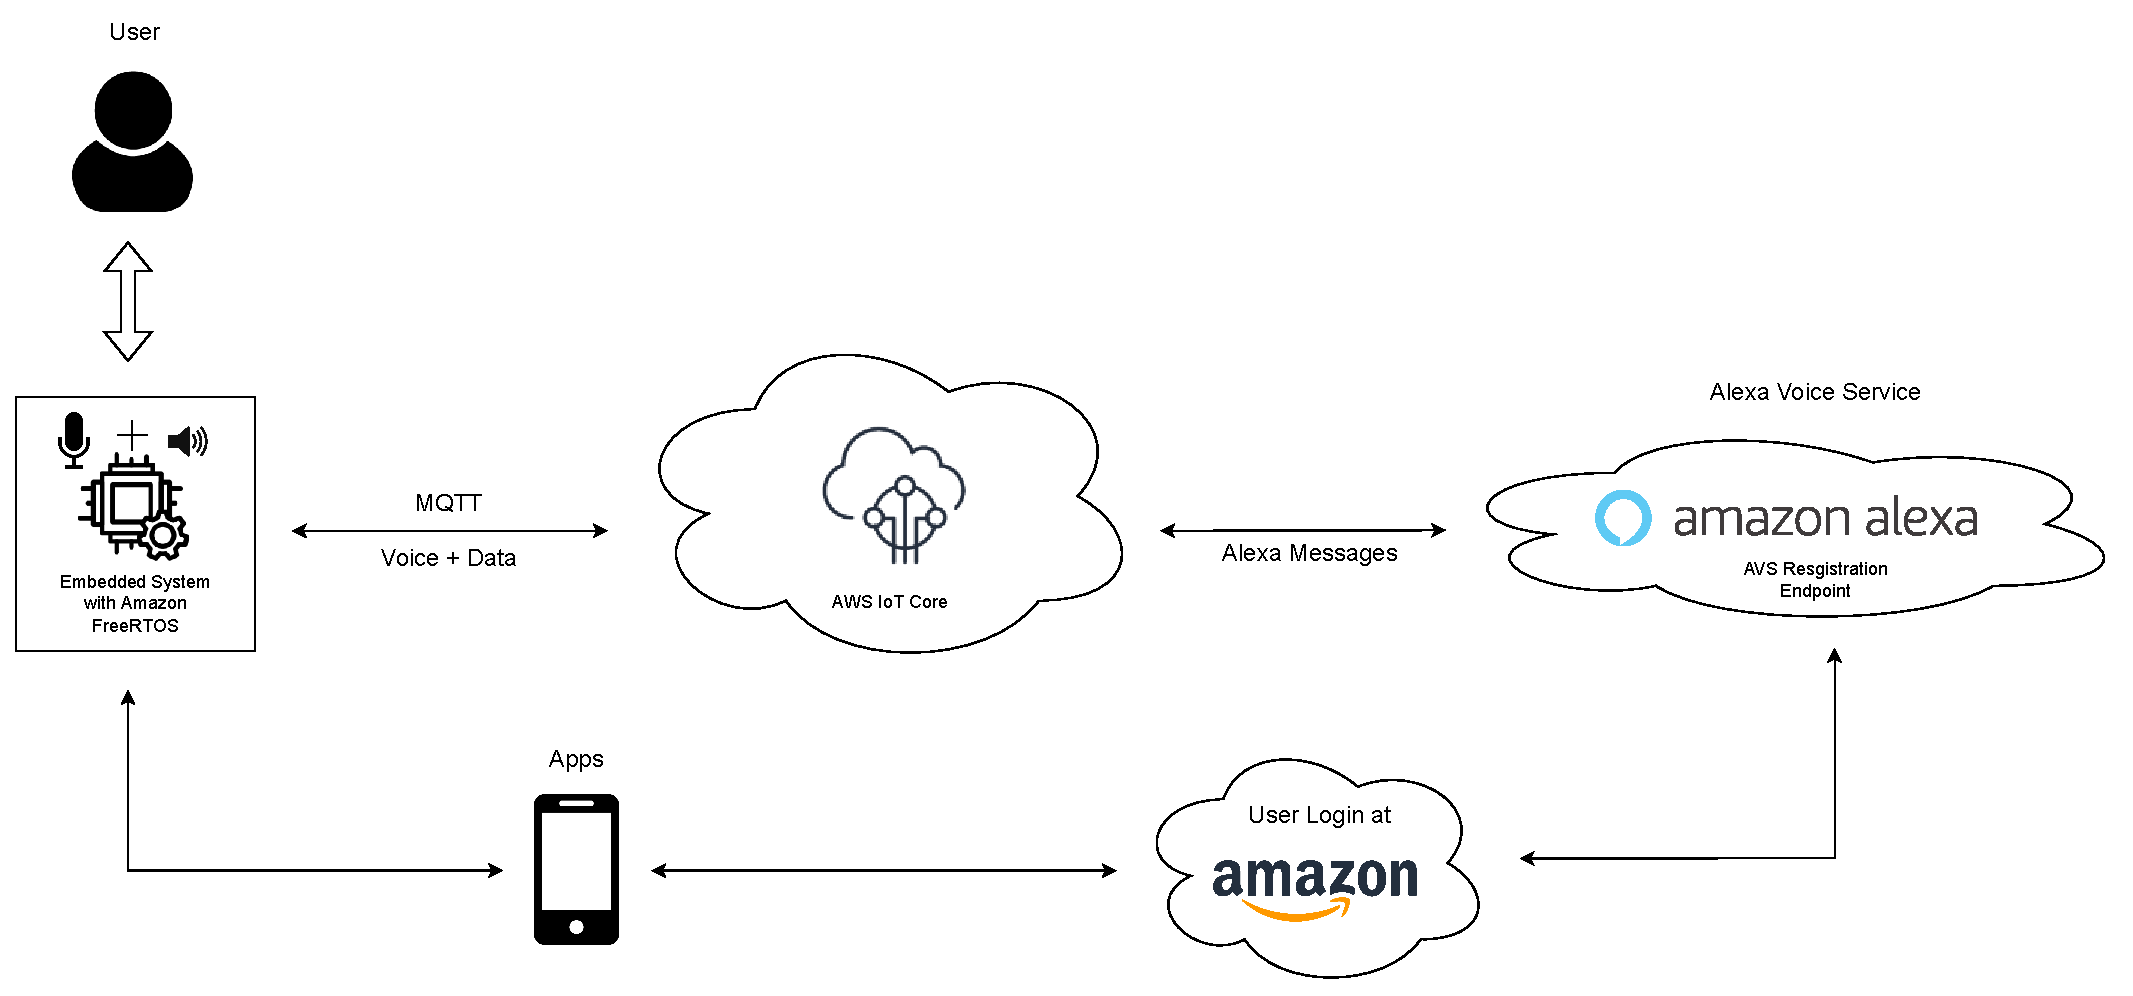
\includegraphics[scale=0.5]{Images/project_diagram.pdf}
	\end{center}
	\legend{Fonte: Autor (2022)}
\end{figure}

\begin{figure}[htb]
	\label{fig_logo_aws}
	\centering
	\begin{minipage}{0.4\textwidth}
		\centering
		\caption{Logo Amazon AWS} \label{fig_logo_aws}
		
\includegraphics[scale=0.2]{Images/logo_aws.pdf}
		\legend{Fonte: Amazon AWS (2022)}
	\end{minipage}
	\hfill
	\begin{minipage}{0.4\textwidth}
		\centering
		\caption{Logo Amazon AWS Lambda} \label{fig_logo_aws_lambda}
		
\includegraphics[scale=0.1]{Images/logo_aws_lambda.pdf}
		\legend{Fonte: Amazon AWS (2022)}
	\end{minipage}
	\hfill
	\begin{minipage}{0.4\textwidth}
		\centering
		\caption{Logo Amazon AWS IoT} \label{fig_logo_aws_iot}
		
\includegraphics[scale=0.2]{Images/logo_aws_iot.pdf}
		\legend{Fonte: Amazon AWS (2022)}
	\end{minipage}
	\hfill
	\begin{minipage}{0.4\textwidth}
		\centering
		\caption{Logo Amazon Alexa} \label{fig_logo_amazon_alexa}
		
\includegraphics[scale=0.7]{Images/logo_amazon_alexa.pdf}
		\legend{Fonte: Amazon Alexa (2022)}
	\end{minipage}
\end{figure}


\section{AWS Lambda}
O AWS Lambda é um serviço de computação sem servidor orientado a eventos que permite a execução em nuvem de códigos (lambdas) de praticamente qualquer tipo de aplicativo ou serviço de \textit{back-end}. Em termos simples, o AWS Lambda permite o acionamento de mais de duzentos serviços da AWS, pagando-se somente pelo recurso utilizado. Nesse projeto, o AWS Lambda será utilizado para a integração do serviço AWS IoT à AVS. A \autoref{fig_logo_aws_lambda} mostra o logo do serviço AWS Lamba.

\section{AWS IoT}
\section{Amazon Alexa}
\section{Trabalhos correlatos}

% ----------------------------------------------------------
% Capítulo 3 - Metodologia
% ----------------------------------------------------------
\chapter{Metodologia}


% ----------------------------------------------------------
% Capítulo 4 - Resultados e Discussão
% ----------------------------------------------------------
\chapter{Resultados e Discussão}

% ----------------------------------------------------------
% Capítulo 5 - Conclusões
% ----------------------------------------------------------
\chapter{Conclusões}

% ----------------------------------------------------------
% ELEMENTOS PÓS-TEXTUAIS
% ----------------------------------------------------------
\postextual

% ----------------------------------------------------------
% Referências bibliográficas
% ----------------------------------------------------------
\bibliography{abntex2-modelo-references}

\end{document}
